\documentclass[8pt]{beamer}
\author{
	Rafik Zitouni\Mark{2}, Jerimie ...\Mark{2}, Aghiles Djoudi\Mark{1}\Mark{2} and Laurent George\Mark{1}	\bigskip\\
	\Mark{1}LIGM/ESIEE Paris, 5 boulevard Descartes, Champs-sur-Marne, France\\
	\Mark{2}SIC/ECE Paris, 37 Quai de Grenelle, 75015 Paris, France\\
	Email:   \{aghiles.djoudi, nawel.zangar, laurent.george\}@esiee.fr, rafik.zitouni@ece.fr
}

% \author{
% 	\IEEEauthorblockN{
% 		Aghiles Djoudi\Mark{1}\Mark{2}, Rafik Zitouni\Mark{2}, Nawel Zangar\Mark{1} and Laurent George\Mark{1}
% 	}
% 	\IEEEauthorblockA{
% 		\Mark{1}LIGM/ESIEE Paris, 5 boulevard Descartes, Champs-sur-Marne, France\\
% 		\Mark{2}SIC/ECE Paris, 37 Quai de Grenelle, 75015 Paris, France\\
% 		Email:   \{aghiles.djoudi, nawel.zangar, laurent.george\}@esiee.fr, rafik.zitouni@ece.fr
% 	}
% }
\setbeamerfont{footnote}{size=\tiny}
\renewcommand{\thefootnote}{\arabic{footnote}}
\setbeamercolor{footnote}{fg=blue}
\setbeamercolor{footnote mark}{fg=blue}


\usepackage{manyfoot}
\newfootnote{A}
\newcounter{footnoteA}
\newcommand{\footnoteA}{%
	\stepcounter{footnoteA}%
	\Footnotemark\thefootnoteA \FootnotetextA{}
}
\renewcommand{\thefootnoteA}{\alph{footnoteA}}


\begin{document}

\firstpage

\section{Introduction}
		\subsection{Context}
		\section{Introduction}

% Context Current needs


% Problematic Current bad state of the research


% Motivation Future good state of the research


% Challenges


% Contribution


% The structure
jjh


\tableofcontent

% Premiere réunion
	%\section{State of the art}
	%	\subsection*{Context}
	%		\begin{frame}{State of the art}{Standardization}
	
	\note{
		\begin{itemize}
			\item Contenu:
			\begin{itemize}
				\item Tableau comparatif (articles connexes/avantages et désavantages)
				\item Les limites de l’existant
				\item Notre travaille traite le meme x que les travaux précidants mais utilise y au lieu de z (xy/xz)
			\end{itemize}
			\item Procedure:
			\begin{itemize}
				\item Lecture en largeur
				\begin{itemize}
					\item Lecture de beaucoup de papiers connexes
					\item Comprendre le domaine
					\item Comprendre les travaux existants
					\item Sélection des travaux intéressants
				\end{itemize}
				\item Lecture en profondeur
				\begin{itemize}
					\item Lecture et analyse des travaux sélectionnés
					\item Descendre jusqu’au détail du détail
					\begin{itemize}
						\item Poser toujours la question pourquoi?
						\item Être capable d’implémenter de suite l’approche.
					\end{itemize}
				\end{itemize}
				\item Situer le travail par rapport à l’existant sur la base de La problématique traitée
				\begin{itemize}
					\item Les critiques faites sur l’existant
					\item Les hypothèses du travail courant
					\item Les objectifs initiales du travail
					\item Les résultats théoriques et expérimentales obtenus
				\end{itemize}
			\end{itemize}
			\item Article:
			\begin{itemize}
				\item Est-ce que le problème est toujours intéressant ?
				\item Est-ce qu'on peux traiter le problème d'une autre manière ?
				\item Est-ce que les hypothèses sont réalistes ?
				\item Est-ce que le travail est applicable dans le contexte actuel ?
				\item Est-ce que tous les aspects du problème ont été traités ?
				\item Existe-t-il d’autres manières pour le résoudre ?
			\end{itemize}
		\end{itemize}
	}
\end{frame}


	%	\subsection{Application protocols}
	%		\begin{frame}{Results}{Comparison with related work}
	\begin{table}
		\begin{tabular}{c|c|c|c|c}
			Paper & A1 & A2 & A3 & A4 \\\hline
				  &    &    &    & \\\hline
				  &    &    &    & \\\hline
				  &    &    &    & \\\hline
				  &    &    &    & 
		\end{tabular}
		\caption{\label{tab:Tableju} An example table.}
	\end{table}
\end{frame}

	%		\begin{frame}{IoT cloud platforms}{State of the art}
%\changefontsizes{8pt}
\begin{table}[h!]
\begin{center}
	\begin{tabulary}{\textwidth}{L|C|C|C|C}
	\bf{Platform}      & \ \bf{COAP} & \bf{XMPP} & \bf{MQTT}\\\hline
	\bf{Arkessa}       &             &           & \ok      \\\hline
	\bf{Axeda}         &             &           &          \\\hline
	\bf{Etherios}      &             &           &          \\\hline
	\bf{LittleBits}    &             &           &          \\\hline
	\bf{NanoService}   & \ok         &           &          \\\hline
	\bf{Nimbits}       &             & \ok       &          \\\hline
	\bf{Ninja blocks}  &             &           &          \\\hline
	\bf{OnePlateformv} & \ok         & \ok       &          \\\hline
	\bf{RealTime.io}   &             &           &          \\\hline
	\bf{SensorCloud}   &             &           &          \\\hline
	\bf{SmartThings}   &             &           &          \\\hline
	\bf{TempoDB}       &             &           &          \\\hline
	\bf{ThingWorx}     &             &           & \ok      \\\hline
	\bf{Xively}        &             &           & \ok      \\\hline
	\bf{Ubidots}       &             &           & \ok      \\\hline
	
	\end{tabulary}
	\caption{\label{tab:IoTPlatforms} IoT cloud platforms and their characteristics}
\end{center}
\end{table}

\end{frame}


	%	\subsection{Service discovery}
	%		\begin{frame}{MDNS}{State of the art}
	\begin{columns}
	
		\begin{column}{0.6\textwidth}
			\begin{itemize}
				\item No need for manual reconfiguration or extra administration
				\item It is able to run without infrastructure
				\item It is able to continue working if failure happens.
				
				\item It inquires names by sending an IP multicast message to all the nodes in the local domain
					\begin{itemize}
						\item Clients asks devices that have the given name to reply back
						\item the target machine receives its name and multicasts its IP @
						\item Devices update their cache with the given name and IP @
					\end{itemize}
				
			\end{itemize}
		\end{column}
		
		\begin{column}{0.4\textwidth}
			\begin{center}
			
				\begin{figure}
					\includegraphics[width=\columnwidth]{mdns.png}
					\caption{\label{fig:mdns} MDNS}
				\end{figure}
				
			\end{center}
			
		\end{column}
	\end{columns}
	
\end{frame}

\begin{frame}{DNS-SD}{State of the art}
	\begin{columns}
		\begin{column}{0.6\textwidth}
		
			\begin{itemize}
				\item Requires zero configuration aids to connect machine
				\item It uses mDNS to send DNS packets to specific multicast addresses through UDP
				\item There are two main steps to process Service Discovery:
					\begin{itemize}
						\item finding host names of required services such as printers
						\item pairing IP addresses with their host names using mDNS
					\end{itemize}
				\item Advantages
					\begin{itemize}
						\item IoT needs an architecture without dependency on a configuration mechanism
						\item smart devices can join the platform or leave it without affecting the behavior of the whole system
					\end{itemize}
				\item Drawbacks
					\begin{itemize}
						\item Need for caching DNS entries
					\end{itemize}
			\end{itemize}
			
		\end{column}
		
		\begin{column}{0.4\textwidth}
			\begin{center}
			
				\begin{figure}
					\includegraphics[width=\columnwidth]{dns-sd.png}
					\caption{\label{fig:dns-sd} DNS-SD}
				\end{figure}
				
			\end{center}
		\end{column}
		
	\end{columns}
	
\end{frame}

\begin{frame}{IoT operating systems}{State of the art}
\changefontsizes{5.3pt}
	\begin{table}[h!]
	\begin{center}
	\begin{tabular}{l|l|c|l|c|c|l|l} % Application protocol
		\bf{OS}      & \bf{Architecture} & \bf{Multi}     & \bf{Scheduling} & \bf{Dynamic}    & \bf{Memory}     & \bf{Network}  & \bf{Virtualization} \\
		\            &                   & \bf{threading} &                 & \bf{Memory}     & \bf{protection} & \bf{Stack} & \bf{and Completion} \\\hline
		\bf{Contiki/Contiki-ng} & Modular        & \ok            & Interrupts      & \ok             & \ko             & uIP          & Serialized          \\
		\            &                   &                & execute w.r.t.  &                 &                 & Rime         & Access              \\\hline
		\bf{MANTIS}  & Modular           & \ko            & Priority        & \ok             & \ko             & At Kernel    & Semaphores.         \\
		\            &                   &                & classes         &                 &                 & COMM layer   &                     \\\hline
		\bf{Nano-RK} & Layered           & \ok            & Monotonic       & \ko             & \ko             & Socket       & Serialized access   \\
		\            &                   &                & harmonized      &                 &                 & abstraction  & semaphores          \\\hline
		\bf{LiteOS}  & Monolithic        & \ok            & Round Robin     & \ok             & \ok             & File         & Synchronization     \\
		\            &                   &                &                 &                 &                 &              & primitives          \\\hline
	\end{tabular}
	\caption{\label{tab:OS} Common operating systems used in IoT environment \cite{al-fuqaha_internet_24}}
	\end{center}
	\end{table}
\end{frame}




	%	\subsection{Network layer}
	%		\begin{frame}{IEEE 802.15.4 topologies}{State of the art}
	\begin{columns}
		
		\begin{column}{0.65\textwidth}
		
			\begin{itemize}
			
				\item Standard topologies to form IEEE 802.15.4e networks are 
					\begin{itemize}
						\item[Star] contains at least one FFD and some RFDs
						\item[Mesh] contains a PAN coordinator and other nodes communicate with each other
						\item[Cluster] consists of a PAN coordinator, a cluster head and normal nodes.
					\end{itemize}
					
				\item The IEEE 802.15.4e standard supports 2 types of network nodes
					\begin{itemize}
						\item[FFD] Full function device: serve as a coordinator
							\begin{itemize}
								\item It is responsible for creation, control and maintenance of the net
								\item It store a routing table in their memory and implement a full MAC
							\end{itemize}
						\item[RFD] Reduced function devices: simple nodes with restricted resources
							\begin{itemize}
								\item They can only communicate with a coordinator
								\item They are limited to a star topology
							\end{itemize}
					\end{itemize}
			\end{itemize}
			
		\end{column}
		
		\begin{column}{0.35\textwidth}
			\begin{center}
			
				\begin{figure}
					\includegraphics[width=\columnwidth]{mac.png}
					\caption{\label{fig:topologies} IEEE 802.15.4 topologies. (a) Star. (b) Mesh. (c) Cluster-tree.}
				\end{figure}
				
			\end{center}
		\end{column}
		
	\end{columns}
	
\end{frame}


	%		\begin{frame}{RPL protocol}{State of the art}
	\begin{columns}
		
		\begin{column}{0.5\textwidth}
		
			\begin{itemize}
				\item Routing over low-power and lossy links (ROLL)
				\item Support minimal routing requirements.
					\begin{itemize}
						\item like multipoint-to-point, point-to-multipoint and point-to-point.
					\end{itemize}
				\item A Destination Oriented Directed Acyclic Graph (DODAG)
					\begin{itemize}
						\item Directed acyclic graph with a single root.
						\item Each node is aware of ts parents 
						\item but not about related children
					\end{itemize}
				\item RPL uses four types of control messages
					\begin{itemize}
						\item DODAG Information Object (DIO)
						\item Destination Advertisement Object (DAO)
						\item DODAG Information Solicitation (DIS)
						\item DAO Acknowledgment (DAO-ACk)
					\end{itemize}
%				\item RPL routers work under one of two modes:
%					\begin{itemize}
%						\item Non-Storing mode
%						\item Storing modes mode
%					\end{itemize}
			\end{itemize}
			
		\end{column}
		
		\begin{column}{0.5\textwidth}
			\begin{center}
			
				\begin{figure}
					\includegraphics[width=\columnwidth]{rpl.png}
					\caption{\label{fig:rpl} RPL protocol}
				\end{figure}
				
				\begin{figure}
					\includegraphics[width=.3\columnwidth]{rpl2.png}
					\caption{\label{fig:rpl2} DODAG messages}
				\end{figure}
				
			\end{center}
		\end{column}
		
	\end{columns}
	
\end{frame}


%\begin{frame}{Results}{State of the art}
%\changefontsizes{5pt}
%\begin{table}[h!]
%\begin{center}
%	\begin{tabulary}{\textwidth}{L|C|C|C|C|C|C|C|C|C}
%	Paper           & Architecture & Availability & Reliability & Mobility & Performance & Management & Scalability & Interoperability & Security\\\hline
%	IoT-A           &              &              &             &          &             &            &             &                  &         \\\hline
%	IoT@Work        &              &              &             &          &             &            &             &                  &         \\\hline
%	EBBITS          &              &              &             &          &             &            &             &                  &         \\\hline
%	BETaas          &              &              &             &          &             &            &             &                  &         \\\hline
%	CALIPSO         &              &              &             &          &             &            &             &                  &         \\\hline
%	VITAL           &              &              &             &          &             &            &             &                  &         \\\hline
%	SENSAI          &              &              &             &          &             &            &             &                  &         \\\hline

%	RERUM           &              &              &             &          &             &            &             &                  &         \\\hline
%	RELEYonIT       &              &              &             &          &             &            &             &                  &         \\\hline

%	IoT6            &              &              &             &          &             &            &             &                  &         \\\hline
%	OpenIoT         &              &              &             &          &             &            &             &                  &         \\\hline
%	Apec IoV        &              &              &             &          &             &            &             &                  &         \\\hline

%	Smart Santander &              &              &             &          &             &            &             &                  &         \\\hline

%	OMA Device      &              &              &             &          &             &            &             &                  &         \\\hline
%	OMA-DM          &              &              &             &          &             &            &             &                  &         \\\hline
%	LWM2M           &              &              &             &          &             &            &             &                  &         \\\hline
%	NETCONF Light   &              &              &             &          &             &            &             &                  &         \\\hline
%	Kura            &              &              &             &          &             &            &             &                  &         \\\hline
%	MASH            &              &              &             &          &             &            &             &                  &         \\\hline

%	IoT-iCore       &              &              &             &          &             &            &             &                  &         \\\hline
%	PROBE-IT        &              &              &             &          &             &            &             &                  &         \\\hline
%	OpenIoT         &              &              &             &          &             &            &             &                  &         \\\hline
%	LinkSmart       &              &              &             &          &             &            &             &                  &         \\\hline

%	IETF SOLACE     &              &              &             &          &             &            &             &                  &         \\\hline
%	BUTLER          &              &              &             &          &             &            &             &                  &         \\\hline
%	Codo            &              &              &             &          &             &            &             &                  &         \\\hline
%	SVELETE         &              &              &             &          &             &            &             &                  &         \\\hline
%	
%	\end{tabulary}
%	\caption{\label{tab:Table54975} An example table.}
%\end{center}
%\end{table}

%\end{frame}


	%	\subsection{Link \& Physical layer}
	%		\begin{frame}{Results}{State of the art}
\changefontsizes{7pt}
\begin{table}[h!]
\begin{center}
	\begin{tabulary}{\textwidth}{L|L|L|L|L}
	\bf{Phy protocol}  & \bf{Radio band (MHz)} & \bf{MAC address} & \bf{Data rate (bps)} & \bf{Scalability} \\\hline
	\bf{IEEE 802.15.4} & 868/915/2400          & TDMA, CSMA/CA    & 20/40/250 K          & 65K nodes  \\\hline
	\bf{BLE}           & 2400                  & TDMA             & 1024K                & 5917 slaves\\\hline
	\bf{EPCglobal}     & 860-960               & ALOHA            & varies 5-640K        & -          \\\hline
%	\bf{LTE-M}         & 700-900               & OFDMA            & 1G (up), 500M (down) & -          \\\hline
	\bf{Z-Wave}        & 868/908/2400          & CSMA/CA          & 40K                  & 232 nodes  \\\hline
	
	\end{tabulary}
	\caption{\label{tab:IoTPlatforms} IoT cloud platforms and their characteristics \cite{al-fuqaha_internet_24}}
\end{center}
\end{table}

\end{frame}


	%		\begin{frame}{Results}{Comparison with related work}
\changefontsizes{6pt}
\begin{table}[h!]
\begin{center}
	\begin{tabular}{l|l|l|l}
	\bf{Characteristics}                           & \bf{6LoWPAN}   & \bf{LoRaWAN}                    & \bf{SigFox}  \\\hline
	\bf{Frequency band}                            & 902-929        & 902-928                         & 902          \\
	\bf{\footnotesize{(MHz)}}                      & 868-868.6      & 863-870 and 434                 & 868          \\\hline
	\bf{Number of channels}                        & 0016 for 2400  & 80             for 915          & 25       \\
	\bf{\footnotesize{(channels for MHz)}}         & 0010 for 915   & 10             for 868 and 780  & \\
	\                                              & 0001 for 868.3 &                                 & \\\hline
	\bf{Channel bandwidth}                         & 0005 for 2400  & 0.125 and 0.50 for 915          & 0.0001-0.0012\\
	\bf{\footnotesize{(MHz)}}                      & 0002 for 915   & 0.125 and 0.25 for 868 and 780  & \\
	\                                              & 0600 for 868.3 &                                 & \\\hline
	\bf{Maximum data rate}                         & 0250 for 2400  & 0.00098-0.0219 for 915          & 0.1-0.6      \\
	\bf{\footnotesize{(kbps for MHz)}}             & 0040 for 915   & 0.250-0.05     for 868 and 780  & \\
	\                                              & 0020 for 868.3 &                                 & \\\hline
%	\bf{Channel modulation}                       & QPSK for 2400  & LoRa           for 915          & BPSK and GFSK\\
%	\                                             & BPSK for 915   & LoRa and GFSK  for 868  and 780 & \\
%	\                                             & BPSK for 868.3 &                                 & \\\hline
	\bf{Channel coding}                            & -085 for 2400  & -137                            & -137         \\
	\bf{\footnotesize{(dBm for MHz)}}              & -092 for 915   &                                 & \\
	\                                              & -092 for 868.3 &                                 & \\\hline
	\bf{Protocol data unit \footnotesize{(bytes)}} & 6+127          & x + (19 to 250)                 & 12+ (0 to 12)\\\hline
	\bf{Channel coding}                            & Direct         & CSS                             & Ultra        \\\hline
	\bf{Transmission range}                        & 10-100 m       & 5-15 km                         & 10-50 km     \\\hline
	\bf{Battery lifetime}                          & 1-2 years      & <10 years                       & <10 years    \\\hline

	\end{tabular}
	\caption{\label{tab:Table54975} LPWan Characteristics \cite{al-kashoash_comparison_2016}}
\end{center}
\end{table}

\end{frame}


%\begin{frame}{Results}{Comparison with related work}
%\changefontsizes{7pt}
%\begin{table}[h!]
%\begin{center}
%	\begin{tabulary}{\textwidth}{L|L|L|L|L|L}
%	\bf{Feature}                     & \bf{Wi-Fi}                                            & \bf{802.11p}                                          & \bf{UMTS}                        & LTE                      & LTE-A                     \\\hline
%	\bf{Channel width MHz}           & 20                                                    & 10                                                    & 5                                & 1.4, 3, 5, 10, 15, 20    & Up to 100                 \\\hline
%	\bf{Frequency band(s) GHz}       & 2.4 , 5.2                                             & 5.86-5.92                                             & 0.7-2.6                          & 0.7-2.69                 & 0.45-4.99                 \\\hline
%	\bf{Bit rate Mb/s}               & 6-54                                                  & 3–27                                                  & 2                                & Up to 300                & Up to 1000                \\\hline
%	\bf{Range km}                    & Up to 0.1                                             & Up to 1                                               & Up to 10                         & Up to 30                 & Up to 30                  \\\hline
%	\bf{Capacity}                    & Medium                                                & Medium                                                & \ko                              & \ok                      & \ok                       \\\hline
%	\bf{Coverage}                    & Intermittent                                          & Intermittent                                          & Ubiquitous                       & Ubiquitous               & Ubiquitous                \\\hline
%	\bf{Mobility support km/h}       & \ko                                                   & Medium                                                & \ok                              & up to 350                & up to 350                 \\\hline
%	\bf{QoS support}                 & EDCA \scriptsize{Enhanced Distributed Channel Access} & EDCA \scriptsize{Enhanced Distributed Channel Access} & QoS classes and bearer selection & QCI and bearer selection & QCI and bearer selection  \\\hline
%	\bf{Broadcast/multicast support} & Native broadcast                                      & Native broadcast                                      & Through MBMS                     & Through eMBMS            & Through eMBMS             \\\hline
%	\bf{V2I support}                 & \ok                                                   & \ok                                                   & \ok                              & \ok                      & \ok                       \\\hline
%	\bf{V2V support}                 & Native (ad hoc)                                       & Native (ad hoc)                                       & \ko                              & \ko                      & Through D2D               \\\hline
%	\bf{Market penetration}          & \ok                                                   & \ko                                                   & \ok                              & \ok                      & \ok                       \\\hline

%	\end{tabulary}
%	\caption{\label{tab:Tableppp} An example table.}
%\end{center}
%\end{table}

%\end{frame}

%\begin{frame}{Results}{Comparison with related work}
%\changefontsizes{7pt}
%\begin{table}[h!]
%\begin{center}
%	\begin{tabulary}{\textwidth}{L|L|L|L|L|L}
%	\bf{Feature}                     & \bf{RFID}                                            & \bf{ZigBee}                                          & \bf{NFC}                        & LTE                      & LTE-A                     \\\hline
%	\bf{Channel width MHz}           & 20                                                    & 10                                                    & 5                                & 1.4, 3, 5, 10, 15, 20    & Up to 100                 \\\hline
%	\bf{Frequency band(s) GHz}       & 2.4 , 5.2                                             & 5.86-5.92                                             & 0.7-2.6                          & 0.7-2.69                 & 0.45-4.99                 \\\hline
%	\bf{Bit rate Mb/s}               & 6-54                                                  & 3–27                                                  & 2                                & Up to 300                & Up to 1000                \\\hline
%	\bf{Range m}                     & 3-10                                                  & 10-100                                                & Up to 6.1                         & Up to 30                 & Up to 30                  \\\hline
%	\bf{Capacity}                    & Medium                                                & Medium                                                & \ko                              & \ok                      & \ok                       \\\hline
%	\bf{Coverage}                    & Intermittent                                          & Intermittent                                          & Ubiquitous                       & Ubiquitous               & Ubiquitous                \\\hline
%	\bf{Mobility support km/h}       & \ko                                                   & Medium                                                & \ok                              & up to 350                & up to 350                 \\\hline
%	\bf{QoS support}                 & EDCA \scriptsize{Enhanced Distributed Channel Access} & EDCA \scriptsize{Enhanced Distributed Channel Access} & QoS classes and bearer selection & QCI and bearer selection & QCI and bearer selection  \\\hline
%	\bf{Broadcast/multicast support} & Native broadcast                                      & Native broadcast                                      & Through MBMS                     & Through eMBMS            & Through eMBMS             \\\hline
%	\bf{V2I support}                 & \ok                                                   & \ok                                                   & \ok                              & \ok                      & \ok                       \\\hline
%	\bf{V2V support}                 & Native (ad hoc)                                       & Native (ad hoc)                                       & \ko                              & \ko                      & Through D2D               \\\hline
%	\bf{Market penetration}          & \ok                                                   & \ko                                                   & \ok                              & \ok                      & \ok                       \\\hline
%	\bf{Data rate}                   & Up to 640 kbps                                        & 250 kbps                                              & 106–424 kbps                              & \ok                      & \ok                       \\\hline
%	\end{tabulary}
%	\caption{\label{tab:Tabliutecv} An example table.}
%\end{center}
%\end{table}

%\end{frame}



%\begin{frame}{Results}{Comparison with related work}

%%\begin{table}[h!]
%%\begin{center}
%	\begin{tabulary}{\textwidth}{|C|C|C|C|C|C|C|C|C|}\hline
%		Preamble & PHDR & PHDRCRC & MHDR & FHDR & FPort & Payload & MIC & CRC \\\hline
%	\end{tabulary}
%%	\caption{\label{tab:Tableijkiikk} An example table.}
%%\end{center}
%%\end{table}

%\end{frame}


%\begin{frame}{Use cases}{Comparison with related work}
%%\changefontsizes{5pt}
%\begin{table}[h!]
%\begin{center}
%	\begin{tabular}{l|l|l|l}
%	\textbf{Use cases}         &  &  & \\\hline
%	Health Monitoring          &  &  & \\\hline
%	Water Distribution         &  &  & \\\hline
%	Electricity Distribution   &  &  & \\\hline
%	Smart Buildings            &  &  & \\\hline
%	Intelligent Transportation &  &  & \\\hline
%	Surveillance               &  &  & \\\hline
%	Environmental Monitoring   &  &  & \\
%	\end{tabular}
%	\caption{\label{tab:IoTUseCase} Use cases \cite{hancke_role_2012}}
%\end{center}
%\end{table}

%\end{frame}


	%\section{Conclusion}
%		\subsection{Conclusion}
\begin{frame}{Conclusion}

	\begin{columns}
		\begin{column}{0.5\textwidth}
%			\newcolumntype{a}{>{\columncolor[gray]{0.8}}c}
			\begin{figure}
				\includegraphics[scale=0.09]{mail.png}
				\caption{\label{fig:g0}Cag.}
			\end{figure}
			\begin{figure}
				\includegraphics[scale=0.09]{mail.png}
				\caption{\label{fig:g1}Cag.}
			\end{figure}
		\end{column}
		\begin{column}{0.5\textwidth}
			\begin{figure}
				\includegraphics[scale=0.09]{mail.png}
				\caption{\label{fig:g2}Cag.}
			\end{figure}
			
			\begin{figure}
				\includegraphics[scale=0.09]{mail.png}
				\caption{\label{fig:g3}Cag.}
			\end{figure}
		\end{column}
	\end{columns}

\end{frame}


%		\begin{frame}[bg]{Challenges}{Conclusion}
	\begin{itemize}
		\item Privacy threats
			\begin{itemize}
				\item Privacy settings
				\item Information propagation
				\item 
			\end{itemize}
		\item Privacy protection
			\begin{itemize}
				\item Privacy settings
				\item I
			\end{itemize}
	\end{itemize}
	\note{L'objectif est de réduire le taux de mortalité}
	\note{L'objectif est de rendre nos route plus sure}
	
	\bey
\end{frame}



\section{State of the art}
		\begin{frame}{State of the art}{Standardization}
	
	\note{
		\begin{itemize}
			\item Contenu:
			\begin{itemize}
				\item Tableau comparatif (articles connexes/avantages et désavantages)
				\item Les limites de l’existant
				\item Notre travaille traite le meme x que les travaux précidants mais utilise y au lieu de z (xy/xz)
			\end{itemize}
			\item Procedure:
			\begin{itemize}
				\item Lecture en largeur
				\begin{itemize}
					\item Lecture de beaucoup de papiers connexes
					\item Comprendre le domaine
					\item Comprendre les travaux existants
					\item Sélection des travaux intéressants
				\end{itemize}
				\item Lecture en profondeur
				\begin{itemize}
					\item Lecture et analyse des travaux sélectionnés
					\item Descendre jusqu’au détail du détail
					\begin{itemize}
						\item Poser toujours la question pourquoi?
						\item Être capable d’implémenter de suite l’approche.
					\end{itemize}
				\end{itemize}
				\item Situer le travail par rapport à l’existant sur la base de La problématique traitée
				\begin{itemize}
					\item Les critiques faites sur l’existant
					\item Les hypothèses du travail courant
					\item Les objectifs initiales du travail
					\item Les résultats théoriques et expérimentales obtenus
				\end{itemize}
			\end{itemize}
			\item Article:
			\begin{itemize}
				\item Est-ce que le problème est toujours intéressant ?
				\item Est-ce qu'on peux traiter le problème d'une autre manière ?
				\item Est-ce que les hypothèses sont réalistes ?
				\item Est-ce que le travail est applicable dans le contexte actuel ?
				\item Est-ce que tous les aspects du problème ont été traités ?
				\item Existe-t-il d’autres manières pour le résoudre ?
			\end{itemize}
		\end{itemize}
	}
\end{frame}


		\subsection{Conclusion}
\begin{frame}{Conclusion}

	\begin{columns}
		\begin{column}{0.5\textwidth}
%			\newcolumntype{a}{>{\columncolor[gray]{0.8}}c}
			\begin{figure}
				\includegraphics[scale=0.09]{mail.png}
				\caption{\label{fig:g0}Cag.}
			\end{figure}
			\begin{figure}
				\includegraphics[scale=0.09]{mail.png}
				\caption{\label{fig:g1}Cag.}
			\end{figure}
		\end{column}
		\begin{column}{0.5\textwidth}
			\begin{figure}
				\includegraphics[scale=0.09]{mail.png}
				\caption{\label{fig:g2}Cag.}
			\end{figure}
			
			\begin{figure}
				\includegraphics[scale=0.09]{mail.png}
				\caption{\label{fig:g3}Cag.}
			\end{figure}
		\end{column}
	\end{columns}

\end{frame}



\section{First contribution}
		\begin{frame}{State of the art}{Standardization}
	
	\note{
		\begin{itemize}
			\item Contenu:
			\begin{itemize}
				\item Tableau comparatif (articles connexes/avantages et désavantages)
				\item Les limites de l’existant
				\item Notre travaille traite le meme x que les travaux précidants mais utilise y au lieu de z (xy/xz)
			\end{itemize}
			\item Procedure:
			\begin{itemize}
				\item Lecture en largeur
				\begin{itemize}
					\item Lecture de beaucoup de papiers connexes
					\item Comprendre le domaine
					\item Comprendre les travaux existants
					\item Sélection des travaux intéressants
				\end{itemize}
				\item Lecture en profondeur
				\begin{itemize}
					\item Lecture et analyse des travaux sélectionnés
					\item Descendre jusqu’au détail du détail
					\begin{itemize}
						\item Poser toujours la question pourquoi?
						\item Être capable d’implémenter de suite l’approche.
					\end{itemize}
				\end{itemize}
				\item Situer le travail par rapport à l’existant sur la base de La problématique traitée
				\begin{itemize}
					\item Les critiques faites sur l’existant
					\item Les hypothèses du travail courant
					\item Les objectifs initiales du travail
					\item Les résultats théoriques et expérimentales obtenus
				\end{itemize}
			\end{itemize}
			\item Article:
			\begin{itemize}
				\item Est-ce que le problème est toujours intéressant ?
				\item Est-ce qu'on peux traiter le problème d'une autre manière ?
				\item Est-ce que les hypothèses sont réalistes ?
				\item Est-ce que le travail est applicable dans le contexte actuel ?
				\item Est-ce que tous les aspects du problème ont été traités ?
				\item Existe-t-il d’autres manières pour le résoudre ?
			\end{itemize}
		\end{itemize}
	}
\end{frame}


		\subsection{Contagion process}
\begin{frame}{... (step 1)}{Methods}

\Itemize{
	\item S = {SF12, BW125, 4/8, 17 dBm}
	\item Input: 
	\Itemize{
		\item Problem: f(x) = {max($x^{2}$), x \in [0,32]}
		\Itemize{
			\item $x_{1}: 01101_{b}$ 
			\item $x_{2}: 11000_{b}$
			\item $x_{3}: 01000_{b}$
			\item $x_{4}: 10011_{b}$
		}
	}

	\item Method: Genetic algorithm
	\Itemize{
		\item Generate a set of random possible solution
		\item Test each solution and see how good it is (ranking)
		\Enumerate{
			\item Remove some bad solutions
			\item Duplicate some good solutions
			\item Make small changes to some of them (Crossover, Mutation)
		}
	}

	\item Output:
	\Itemize{
			\item $x_{1}$: 01101  (169)  (14.4)
			\item $x_{2}$: 11000  (576)  (49.2)
			\item $x_{3}$: 01000  (64 )  (5.5)
			\item $x_{4}$: 10011  (361)  (30.9)
	}
}
\end{frame}

%\note{
%	\begin{itemize}
%		\item Contenu:
%		\begin{itemize}
%			\item L’approche doit être soigneusement détaillée
%			\item Motiver les étapes, les hypothèses, le contexte
%			\item Dérouler un exemple si nécessaire
%			\item Illustrer par des schémas et figures
%			\item Se concentrer sur les aspects où l’approche apporte une contribution
%			\item Montrer comment on est différent de l’existant
%		\end{itemize}
%		\item Conseils:
%		\begin{itemize}
%			\item Présentation de l'approche utilisée pour résoudre le problème posé: approche(contrainte, parametre du probleme) = solution
%			\begin{itemize}
%				\item Justification du choix de l'approche
%				\item Description générale de l’approche comme une boite noir
%				\begin{itemize}
%					\item Entrées, Sorties, Contraintes, Hypothèses
%				\end{itemize}
%				\item Description détaillée de la solution du problème
%				\begin{itemize}
%					\item Description détaillée des étapes: paramètre -> étape1 -> étape2, ... -> solution
%					\item Modélisation des objets manipulés
%				\end{itemize}
%			\end{itemize}
%			\item Mise en œuvre des hypothèses
%			\item Description de la solution du problème
%		\end{itemize}
%		\item Conseils 2:
%		\begin{itemize}
%			\item Utilisez un exemple pour le dérouler tout au long des étapes de l’approche
%			\item Ne parlez dans ce chapitre que de votre travail, ce qu’ont fait les autres est dans l’état de l’art
%			\item Insistez sur les parties où vous apportez des contributions
%			\item Montrez comment votre travail est différent des autres
%			\item Montrez les modules/algorithmes pris de l’existant, ne réinventez pas la roue.
%			\item le lecteur doit pouvoir reproduire les résultats en appliquant la même approche.
%		\end{itemize}
%	\end{itemize}
%}

\begin{frame}{... (step 2)}{Methods}
	\Itemize{
		\item 
		\item 
	}
\end{frame}

\begin{frame}{... (step 3)}{Methods}
	\Itemize{
		\item 
		\item 
	}
\end{frame}

\begin{frame}{... (step 4)}{Methods}
	\Itemize{
		\item 
		\item 
	}
\end{frame}

\begin{frame}{Results}{Comparison}
	\begin{table}[h!]
	\scriptsize
		\begin{tabulary}{\textwidth}{L|L|L|L|L}
		\  &  &  &  &  \\\hline
		\  &  &  &  &  \\\hline
		\  &  &  &  &  \\\hline
		\  &  &  &  &  \\\hline
		\  &  &  &  &  \\\hline
		\end{tabulary}
	\caption{\label{tab:} }
	\end{table}
\end{frame}


		\subsection{Experimentation}
\begin{frame}{Experimentation}{Experimentation}
	\begin{itemize}
		\item Privacy threats
			\begin{itemize}
				\item Privacy settings
				\item Information propagation
				\item 
			\end{itemize}
		\item Privacy protection
			\begin{itemize}
				\item Privacy settings
				\item I
			\end{itemize}
	\end{itemize}
	
\end{frame}


		\begin{frame}{Results}{Comparison}

	\Columns{0.5}{0.5}{
		\begin{figure}
			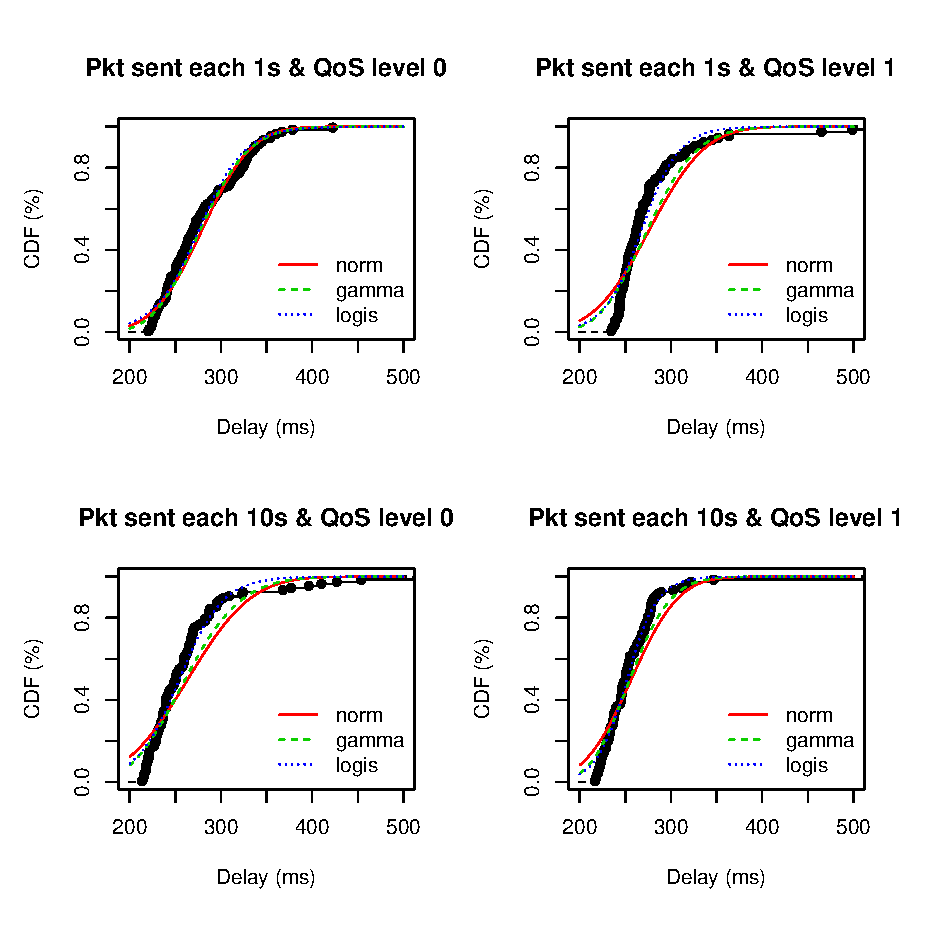
\includegraphics[width=\columnwidth]{distributions_v3.eps}
			\caption{\label{fig:distributions_v3.eps}Distributions}
		\end{figure}
	}{
		\begin{figure}
			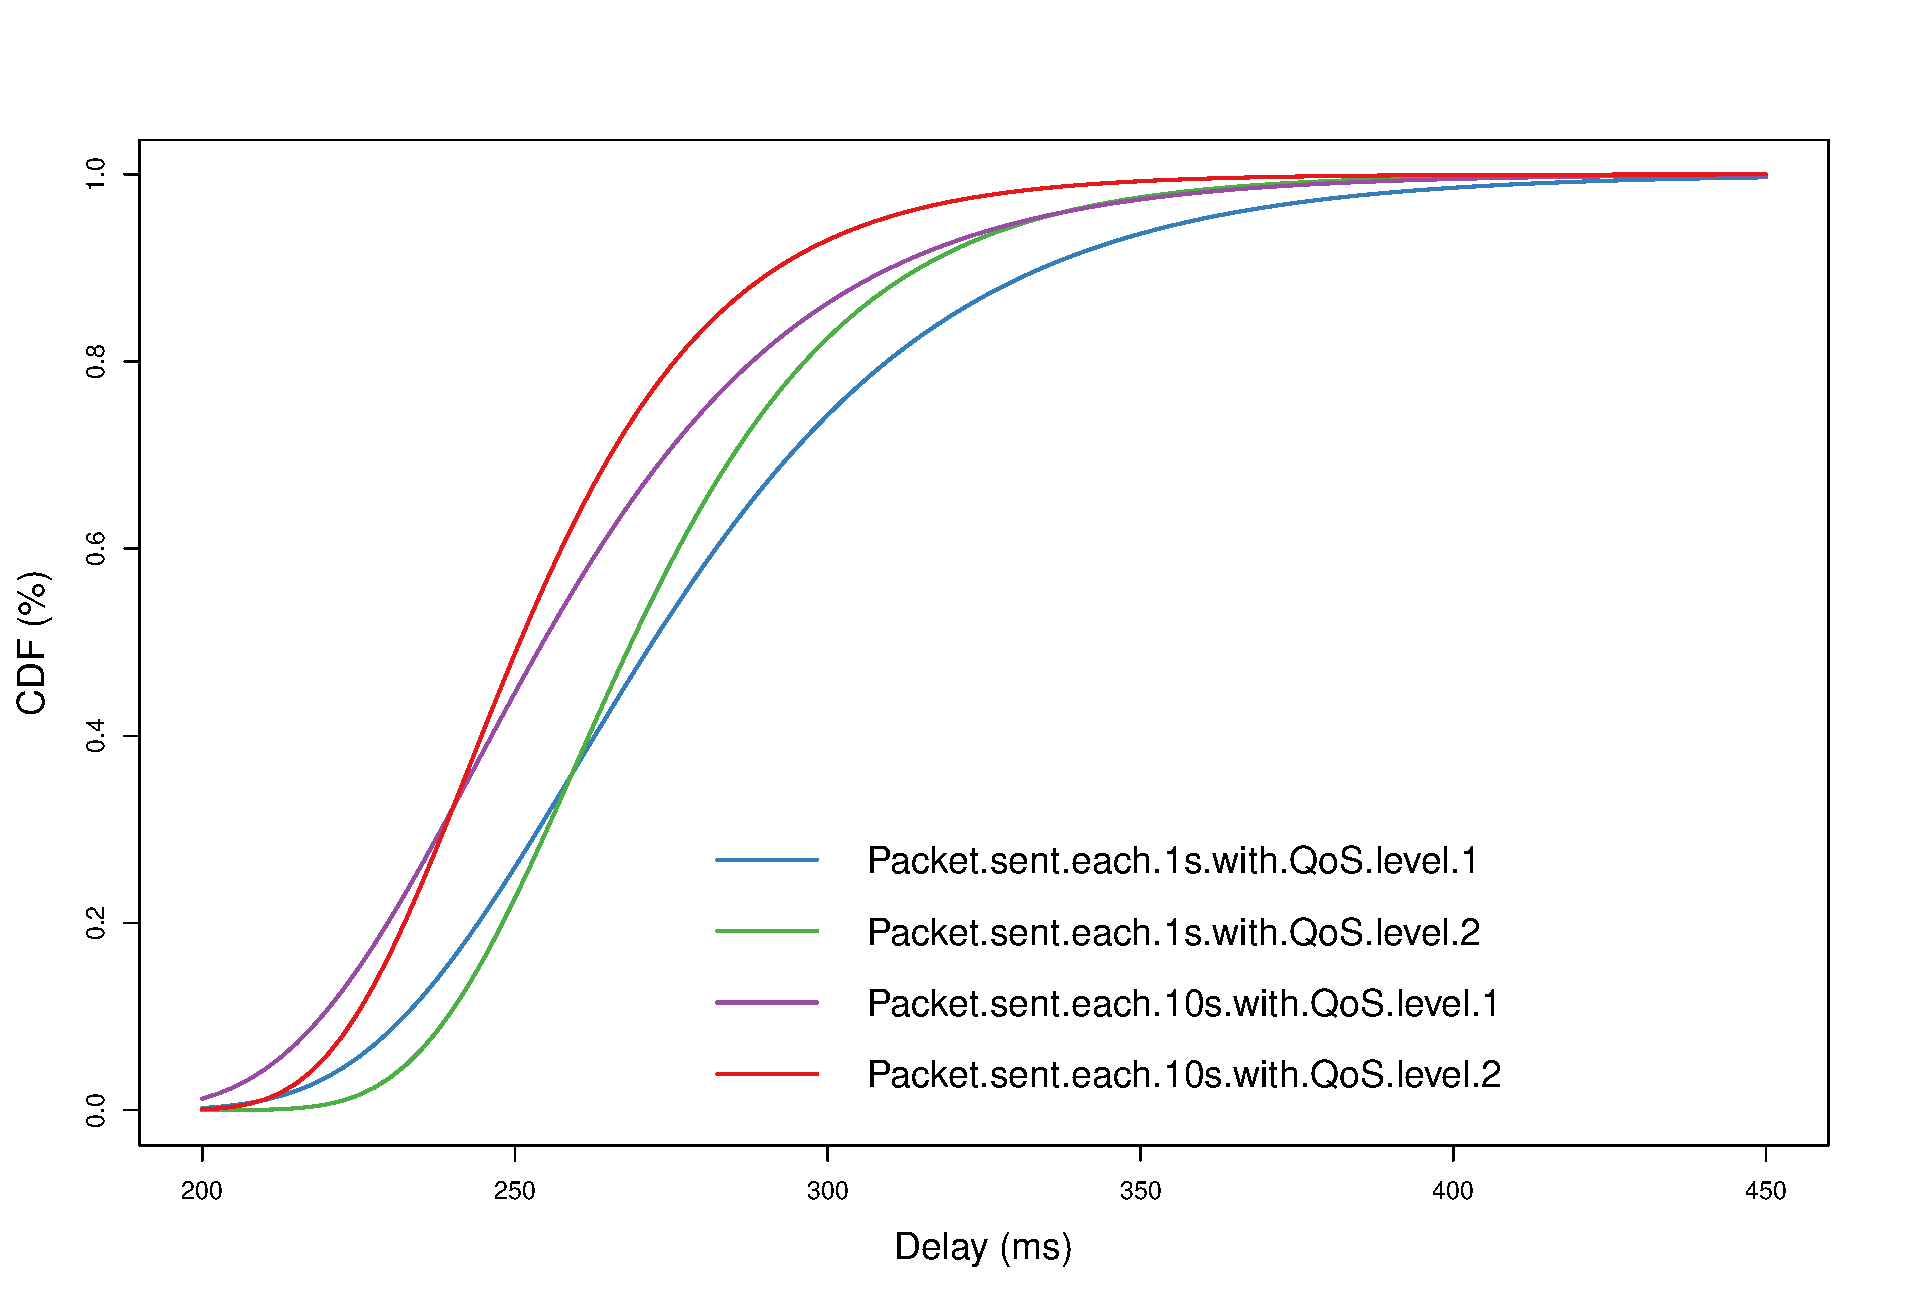
\includegraphics[width=\columnwidth]{res/cdf_v3.eps}
			\caption{\label{fig:cdf_v3.eps}CDF comparison}
		\end{figure}
	}
	
\end{frame}


		\subsection{Conclusion}
\begin{frame}{Conclusion}

	\begin{columns}
		\begin{column}{0.5\textwidth}
%			\newcolumntype{a}{>{\columncolor[gray]{0.8}}c}
			\begin{figure}
				\includegraphics[scale=0.09]{mail.png}
				\caption{\label{fig:g0}Cag.}
			\end{figure}
			\begin{figure}
				\includegraphics[scale=0.09]{mail.png}
				\caption{\label{fig:g1}Cag.}
			\end{figure}
		\end{column}
		\begin{column}{0.5\textwidth}
			\begin{figure}
				\includegraphics[scale=0.09]{mail.png}
				\caption{\label{fig:g2}Cag.}
			\end{figure}
			
			\begin{figure}
				\includegraphics[scale=0.09]{mail.png}
				\caption{\label{fig:g3}Cag.}
			\end{figure}
		\end{column}
	\end{columns}

\end{frame}


		\begin{frame}[bg]{Challenges}{Conclusion}
	\begin{itemize}
		\item Privacy threats
			\begin{itemize}
				\item Privacy settings
				\item Information propagation
				\item 
			\end{itemize}
		\item Privacy protection
			\begin{itemize}
				\item Privacy settings
				\item I
			\end{itemize}
	\end{itemize}
	\note{L'objectif est de réduire le taux de mortalité}
	\note{L'objectif est de rendre nos route plus sure}
	
	\bey
\end{frame}



\section{Second contribution}
		\begin{frame}{State of the art}{Standardization}
	
	\note{
		\begin{itemize}
			\item Contenu:
			\begin{itemize}
				\item Tableau comparatif (articles connexes/avantages et désavantages)
				\item Les limites de l’existant
				\item Notre travaille traite le meme x que les travaux précidants mais utilise y au lieu de z (xy/xz)
			\end{itemize}
			\item Procedure:
			\begin{itemize}
				\item Lecture en largeur
				\begin{itemize}
					\item Lecture de beaucoup de papiers connexes
					\item Comprendre le domaine
					\item Comprendre les travaux existants
					\item Sélection des travaux intéressants
				\end{itemize}
				\item Lecture en profondeur
				\begin{itemize}
					\item Lecture et analyse des travaux sélectionnés
					\item Descendre jusqu’au détail du détail
					\begin{itemize}
						\item Poser toujours la question pourquoi?
						\item Être capable d’implémenter de suite l’approche.
					\end{itemize}
				\end{itemize}
				\item Situer le travail par rapport à l’existant sur la base de La problématique traitée
				\begin{itemize}
					\item Les critiques faites sur l’existant
					\item Les hypothèses du travail courant
					\item Les objectifs initiales du travail
					\item Les résultats théoriques et expérimentales obtenus
				\end{itemize}
			\end{itemize}
			\item Article:
			\begin{itemize}
				\item Est-ce que le problème est toujours intéressant ?
				\item Est-ce qu'on peux traiter le problème d'une autre manière ?
				\item Est-ce que les hypothèses sont réalistes ?
				\item Est-ce que le travail est applicable dans le contexte actuel ?
				\item Est-ce que tous les aspects du problème ont été traités ?
				\item Existe-t-il d’autres manières pour le résoudre ?
			\end{itemize}
		\end{itemize}
	}
\end{frame}


		\subsection{Contagion process}
\begin{frame}{... (step 1)}{Methods}

\Itemize{
	\item S = {SF12, BW125, 4/8, 17 dBm}
	\item Input: 
	\Itemize{
		\item Problem: f(x) = {max($x^{2}$), x \in [0,32]}
		\Itemize{
			\item $x_{1}: 01101_{b}$ 
			\item $x_{2}: 11000_{b}$
			\item $x_{3}: 01000_{b}$
			\item $x_{4}: 10011_{b}$
		}
	}

	\item Method: Genetic algorithm
	\Itemize{
		\item Generate a set of random possible solution
		\item Test each solution and see how good it is (ranking)
		\Enumerate{
			\item Remove some bad solutions
			\item Duplicate some good solutions
			\item Make small changes to some of them (Crossover, Mutation)
		}
	}

	\item Output:
	\Itemize{
			\item $x_{1}$: 01101  (169)  (14.4)
			\item $x_{2}$: 11000  (576)  (49.2)
			\item $x_{3}$: 01000  (64 )  (5.5)
			\item $x_{4}$: 10011  (361)  (30.9)
	}
}
\end{frame}

%\note{
%	\begin{itemize}
%		\item Contenu:
%		\begin{itemize}
%			\item L’approche doit être soigneusement détaillée
%			\item Motiver les étapes, les hypothèses, le contexte
%			\item Dérouler un exemple si nécessaire
%			\item Illustrer par des schémas et figures
%			\item Se concentrer sur les aspects où l’approche apporte une contribution
%			\item Montrer comment on est différent de l’existant
%		\end{itemize}
%		\item Conseils:
%		\begin{itemize}
%			\item Présentation de l'approche utilisée pour résoudre le problème posé: approche(contrainte, parametre du probleme) = solution
%			\begin{itemize}
%				\item Justification du choix de l'approche
%				\item Description générale de l’approche comme une boite noir
%				\begin{itemize}
%					\item Entrées, Sorties, Contraintes, Hypothèses
%				\end{itemize}
%				\item Description détaillée de la solution du problème
%				\begin{itemize}
%					\item Description détaillée des étapes: paramètre -> étape1 -> étape2, ... -> solution
%					\item Modélisation des objets manipulés
%				\end{itemize}
%			\end{itemize}
%			\item Mise en œuvre des hypothèses
%			\item Description de la solution du problème
%		\end{itemize}
%		\item Conseils 2:
%		\begin{itemize}
%			\item Utilisez un exemple pour le dérouler tout au long des étapes de l’approche
%			\item Ne parlez dans ce chapitre que de votre travail, ce qu’ont fait les autres est dans l’état de l’art
%			\item Insistez sur les parties où vous apportez des contributions
%			\item Montrez comment votre travail est différent des autres
%			\item Montrez les modules/algorithmes pris de l’existant, ne réinventez pas la roue.
%			\item le lecteur doit pouvoir reproduire les résultats en appliquant la même approche.
%		\end{itemize}
%	\end{itemize}
%}

\begin{frame}{... (step 2)}{Methods}
	\Itemize{
		\item 
		\item 
	}
\end{frame}

\begin{frame}{... (step 3)}{Methods}
	\Itemize{
		\item 
		\item 
	}
\end{frame}

\begin{frame}{... (step 4)}{Methods}
	\Itemize{
		\item 
		\item 
	}
\end{frame}

\begin{frame}{Results}{Comparison}
	\begin{table}[h!]
	\scriptsize
		\begin{tabulary}{\textwidth}{L|L|L|L|L}
		\  &  &  &  &  \\\hline
		\  &  &  &  &  \\\hline
		\  &  &  &  &  \\\hline
		\  &  &  &  &  \\\hline
		\  &  &  &  &  \\\hline
		\end{tabulary}
	\caption{\label{tab:} }
	\end{table}
\end{frame}


		\subsection{Experimentation}
\begin{frame}{Experimentation}{Experimentation}
	\begin{itemize}
		\item Privacy threats
			\begin{itemize}
				\item Privacy settings
				\item Information propagation
				\item 
			\end{itemize}
		\item Privacy protection
			\begin{itemize}
				\item Privacy settings
				\item I
			\end{itemize}
	\end{itemize}
	
\end{frame}


		\begin{frame}{Results}{Comparison}

	\Columns{0.5}{0.5}{
		\begin{figure}
			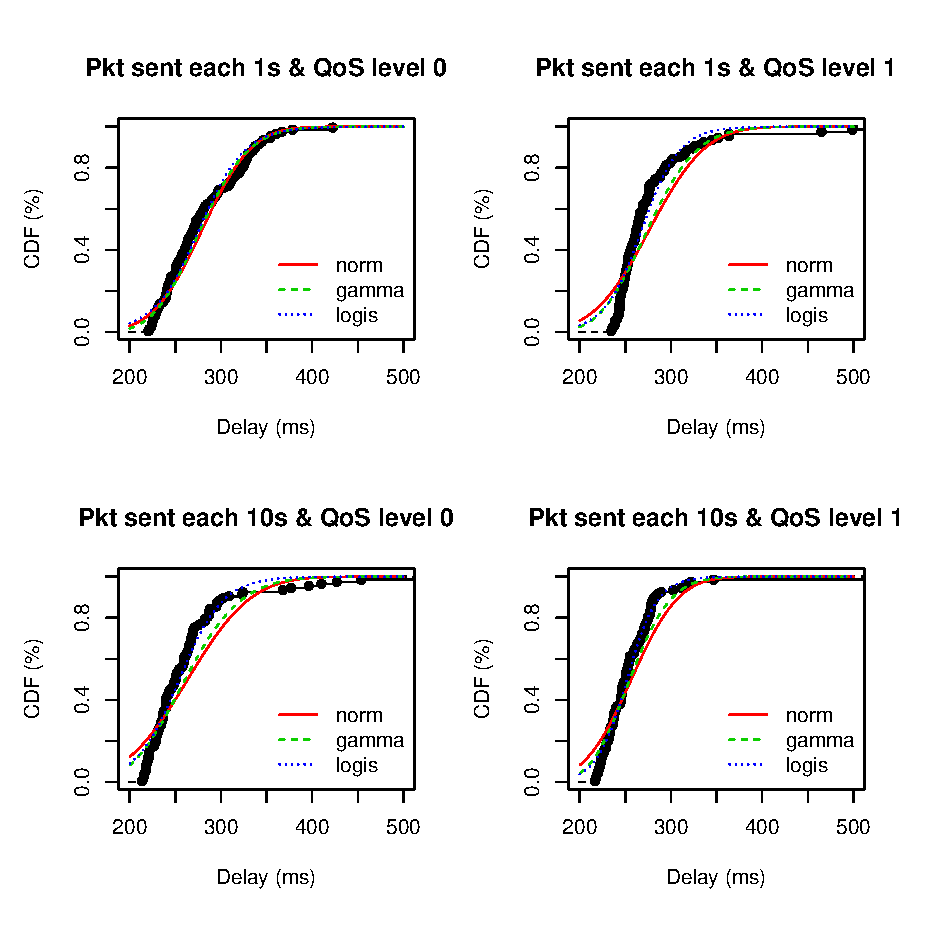
\includegraphics[width=\columnwidth]{distributions_v3.eps}
			\caption{\label{fig:distributions_v3.eps}Distributions}
		\end{figure}
	}{
		\begin{figure}
			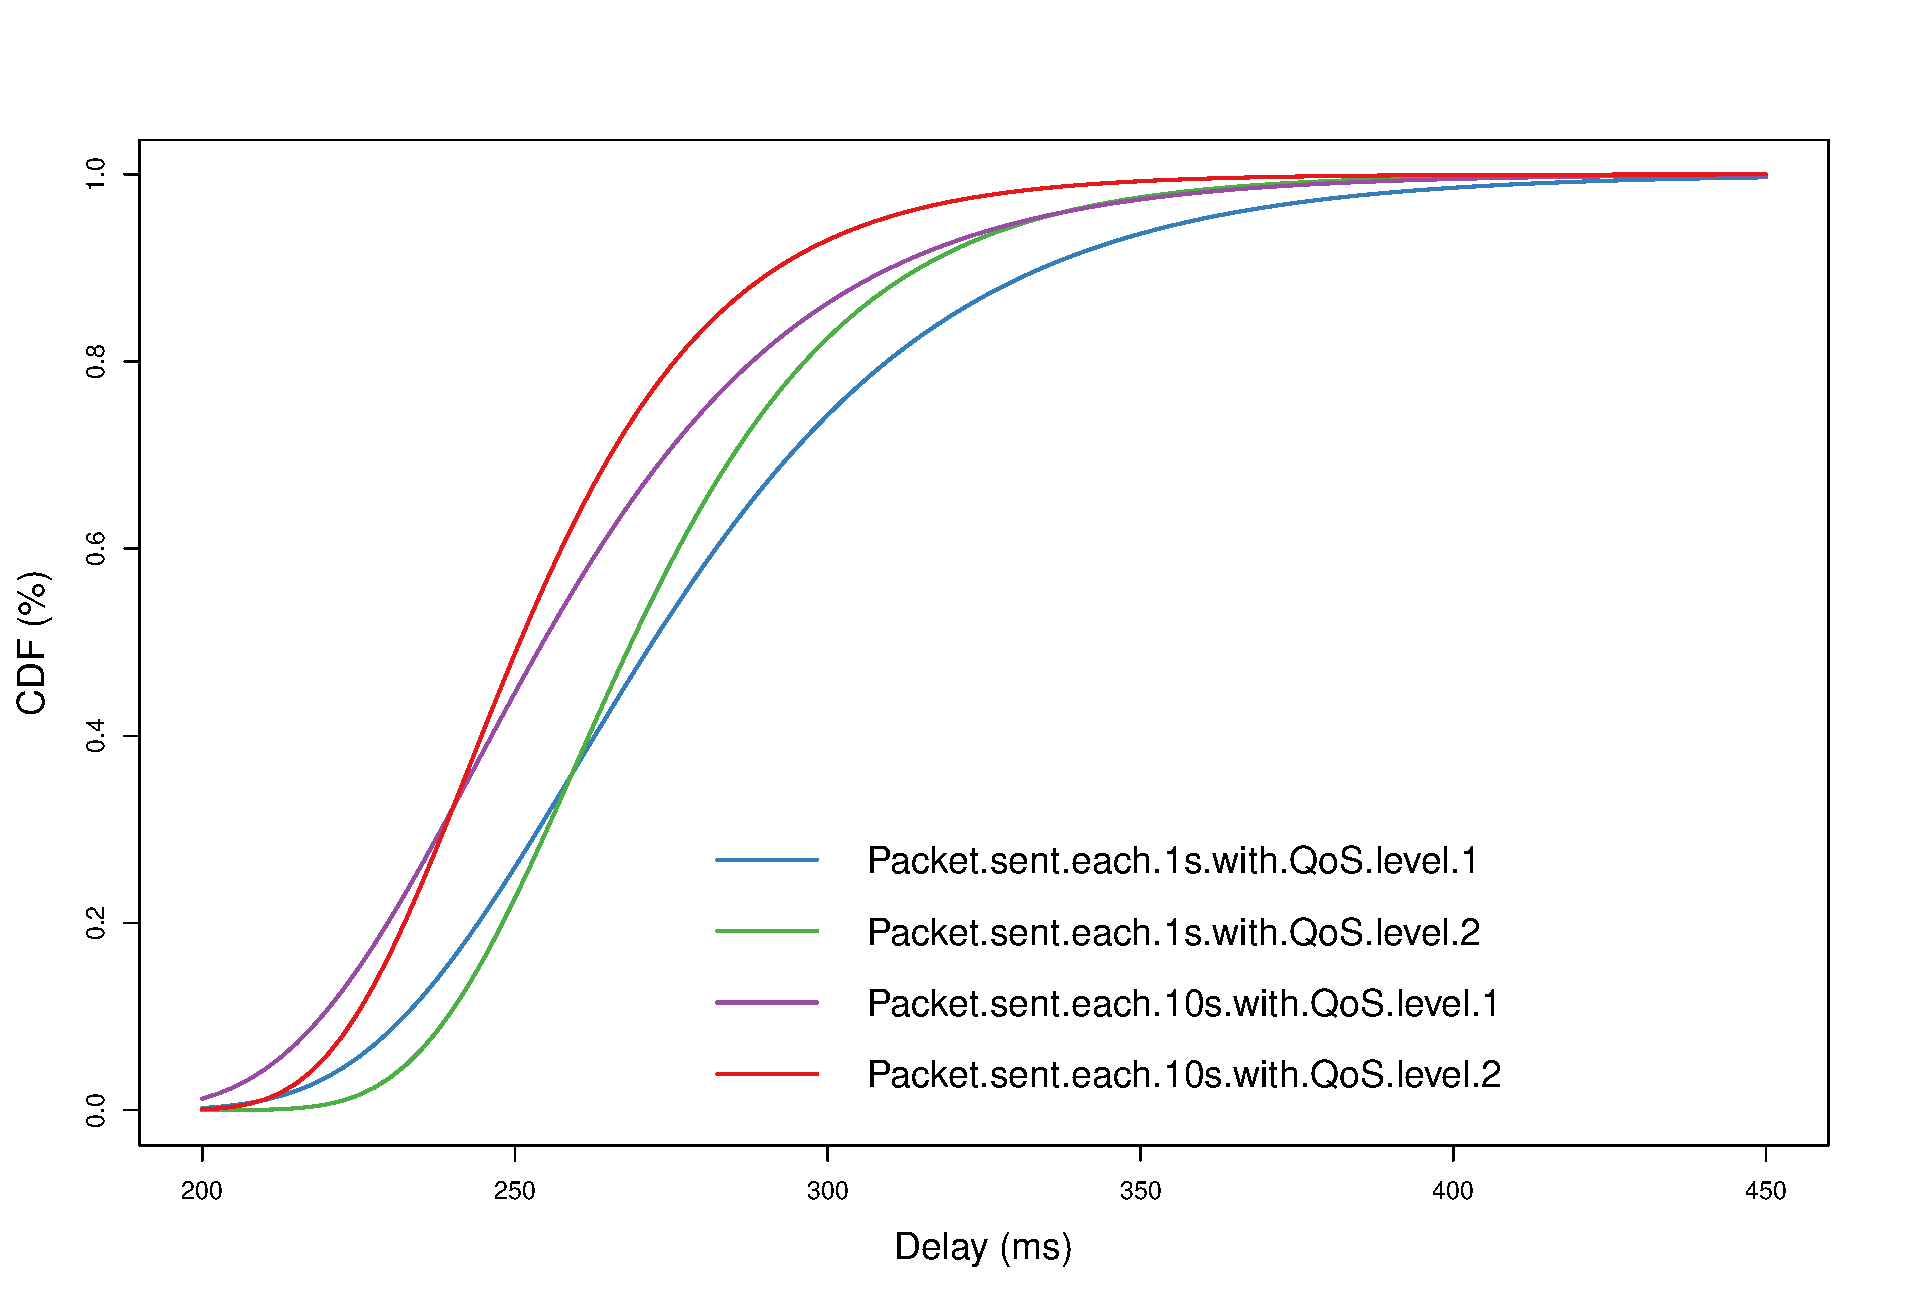
\includegraphics[width=\columnwidth]{res/cdf_v3.eps}
			\caption{\label{fig:cdf_v3.eps}CDF comparison}
		\end{figure}
	}
	
\end{frame}


		\subsection{Conclusion}
\begin{frame}{Conclusion}

	\begin{columns}
		\begin{column}{0.5\textwidth}
%			\newcolumntype{a}{>{\columncolor[gray]{0.8}}c}
			\begin{figure}
				\includegraphics[scale=0.09]{mail.png}
				\caption{\label{fig:g0}Cag.}
			\end{figure}
			\begin{figure}
				\includegraphics[scale=0.09]{mail.png}
				\caption{\label{fig:g1}Cag.}
			\end{figure}
		\end{column}
		\begin{column}{0.5\textwidth}
			\begin{figure}
				\includegraphics[scale=0.09]{mail.png}
				\caption{\label{fig:g2}Cag.}
			\end{figure}
			
			\begin{figure}
				\includegraphics[scale=0.09]{mail.png}
				\caption{\label{fig:g3}Cag.}
			\end{figure}
		\end{column}
	\end{columns}

\end{frame}


		\begin{frame}[bg]{Challenges}{Conclusion}
	\begin{itemize}
		\item Privacy threats
			\begin{itemize}
				\item Privacy settings
				\item Information propagation
				\item 
			\end{itemize}
		\item Privacy protection
			\begin{itemize}
				\item Privacy settings
				\item I
			\end{itemize}
	\end{itemize}
	\note{L'objectif est de réduire le taux de mortalité}
	\note{L'objectif est de rendre nos route plus sure}
	
	\bey
\end{frame}



\section{Conclusion}
		\input{src/2_conclusion}

%\alltableofcontent

\frameBibliography
\end{document}


